\documentclass{article}
\linespread{1.25}

\usepackage[top = 1cm, right=2cm, left=2cm]{geometry}
\usepackage{sectsty}
\usepackage{amsmath}

\usepackage{tikz}
\usetikzlibrary{trees}

\usepackage{graphicx}
\usepackage{xepersian}
\settextfont{B Nazanin}
\setlatinmonofont{CMU Serif}
%\setlatinmonofont{Times New Roman}
\setlatintextfont{Times New Roman}

% Set Latin Modern font for the bullets in itemizea
\newfontfamily\latinbullet{Latin Modern Roman}
\sectionfont{\fontsize{12}{15}\selectfont}
\DeclareMathOperator*{\argmax}{arg\,max}

\title{پاسخ تکلیف 
	\lr{Decision Tree}
}
\author{درس یادگیری ماشین}
\date{
	امیرحسین ابوالحسنی\\
	400405003
	}
	
	
% Commands
\newcommand{\column}[1]{\lr{\textit{#1}}}
\renewcommand{\labelitemi}{{\latinbullet\textbullet}} % Use the bullet from Latin Modern font
\newcommand{\tf}[1]{\text{\lr{#1}}}

\begin{document}
	\maketitle
	
	\begin{latin}
		\section{Suppose there is an attribute, "A," that consists of random values, and these
			values do not have any correlation with the class labels. Additionally, assume that
			"A" has a sufficient number of distinct values such that no two instances in the
			training dataset share the same value for "A." What would be the outcome if a
			decision tree is built using this attribute? What challenges or issues might arise in
			this scenario?}
	\end{latin}
	\noindent
	\subsection*{پاسخ}
	\subsubsection*{قسمت اول}
	با توجه به الگوریتم 
	\lr{ID3}،
	در ابتدا 
	\lr{information gain}
	ناشی از هر ویژگی را سنجیده و آن ویژگی که بیشترین 
	\lr{gain}
	را دارد انتخاب می‌کنیم\\
	(تعداد کلاس‌های هدف = \lr{k}):
	\[
	Gain(S, A) = Entropy(S) - \sum_{v \in A} \frac{| S_v |}{| S |}Entropy(S_v)
	\] 
	\[
	Entropy(S_v) = -\sum_{v} p_v\log (p_v) = -(P(S_v = 0) \log P(S_v = 0) + P(S_v = 1) \log P(S_v = 1) + \dots‌+ P(S_v = k) \log p(S_v = k))
	\]
	به علت یکتایی این ویژگی(کلید اصلی بودن) برای هر نمونه، همه ترم‌های $P(S_v = l) \log P(S_v = l)$ برابر با صفر می‌شود.  زیرا 
	\[
	P(S_v = l) = 0
	\]
	یا
	\[
	P(S_v = l) = 1
	\]
	 در نتیجه یکی از مضرب ها 0 خواهد شد و کل ترم‌ را 0 خواهد کرد. بدین صورت است که نتیجه می‌گیریم:
	\[
	Entropy(S_v) = 0
	\]
	و این ویژگی برای ریشه انتخاب می‌گردد:
	\[
	\argmax ~ \{Gain(S_v) |\forall A \in \text{\lr{Header}}\} = A
	\]
	در نتیجه این کار، ارتفاع درخت 1 شده و به تعداد مقادیر ویژگی 
	\lr{A}،
شاخه خواهیم داشت.
		\subsubsection*{قسمت دوم}
		در صورتی که این ویژگی با ویژگی هدف هیچ رابطه‌ای نداشته باشد، استفاده از این ویژگی کاملا اشتباه است و منجر به 
		\lr{overfit}
		می‌شود. زیرا عملا هیچ جایی برای 
		\lr{generalization}
		باقی نمی‌ماند.
	\begin{latin}
		\section{Answer the questions according to the following dataset:}
		\begin{center}
			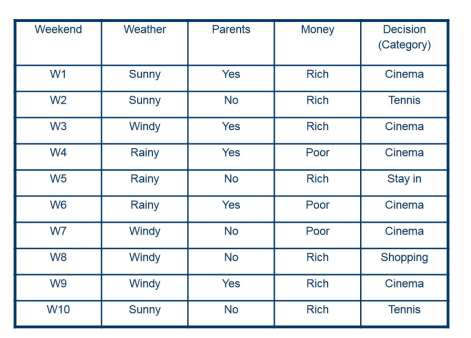
\includegraphics{figs/Dataset_image.png}
		\end{center}
		
		\subsection{Create a decision tree model using the given dataset to predict the value
			of the final column, using all other columns as input features except for
			the first one(weekend). Clearly explain each step of the process, including
			your calculations, reasoning, and decisions made while constructing the
			tree. What is the model's overall classification accuracy?}
	\end{latin}
	1 - \lr{Root Node}
	\begin{latin}
		\textbf{Decision}
		\begin{center}
			\begin{tabular}{|c|c|c|c|c|}
				\hline
				Cinema & Tennis & Stay in & Shopping\\
				\hline
				\hline
				 6 & 2 & 1 & 1\\
				\hline
			\end{tabular}
		\end{center}
	\end{latin}
	\vspace{5pt}
	\[
	Entropy(S) = -\sum_{v \in S} p_v\log (p_v)
	\]
	\[
	Entropy(S) = -( 0.6 \times -0.73 + 0.2 \times -2.32‌ + 0.1 \times -3.32 + 0.1 \times -3.32) = 1.56
	\]
	\begin{latin}
		\textbf{Money}
		\begin{center}
			\begin{tabular}{|c|c|c|c|c|c|}
				\hline
				Value & Cinema & Tennis & Stay in & Shopping\\
				\hline
				\hline
				Rich & ‌3& 2 & 1 & 1\\
				\hline
				Poor & 3 & 0 & 0 & 0\\
				\hline
			\end{tabular}
		\end{center}
	\end{latin}
	\vspace{5pt}
	\[
	Entropy(S_{\text{\lr{v}}}) = -\sum_{v \in S} p_v\log (p_v)
	\]
	\[
	Entropy(S_{\tf{Rich}}) = -(0.42 \times -1.25 + 0.28 \times -1.83 + 0.14 \times -2.83 + 0.14 \times -2.83) = 1.82
	\]
	\[
	Entropy(S_{\tf{Poor}}) = -(0.42 \times -1.25) = 0.52
	\]
	\vspace{10pt}
	\[
	Gain(S, \tf{Money}) = Entropy(S) - \sum_{v \in \tf{Money}} \frac{| S_v |}{| S |}Entropy(S_v)
	\] 
	\[
	\sum_{v \in \tf{Money}} \frac{| S_v |}{| S |}Entropy(S_v) = \frac{7}{10} \times 1.82 + \frac{3}{10} \times 0.52 = 1.43
	\]
	\[
	Gain(S, \tf{Money}) = 1.56 - 1.43 = 0.13
	\]
	\begin{latin}
		\textbf{Parents}
		\begin{center}
			\begin{tabular}{|c|c|c|c|c|c|}
				\hline
				Value & Cinema & Tennis & Stay in & Shopping\\
				\hline
				\hline
				Yes & ‌5& 0 & 0 & 0\\
				\hline
				No & 1 & 2 & 1 & 1\\
				\hline
			\end{tabular}
		\end{center}
	\end{latin}
	\vspace{5pt}
	\[
	Entropy(S_{\tf{v}}) = -\sum_{v \in S} p_v\log (p_v)
	\]
	\[
	Entropy(S_{\tf{Yes}}) = -(\frac{5}{5} \times 0) = 0
	\]
	\[
	Entropy(S_{\tf{No}}) = -(0.2 \times -2.32 + 0.4 \times -1.32 + 0.2 \times -2.32 + 0.2 \times -2.32) = 1.92
	\]
	\vspace{10pt}
	\[
	Gain(S, \tf{Parents}) = Entropy(S) - \sum_{v \in \tf{Parents}} \frac{| S_v |}{| S |}Entropy(S_v)
	\] 
	\[
	\sum_{v \in \tf{Parents}} \frac{| S_v |}{| S |}Entropy(S_v) = \frac{5}{10} \times 0 + \frac{5}{10} \times 1.92 = 0.96
	\]
	\[
	Gain(S, \tf{Parents}) = 1.56 - 0.96 = 0.6
	\]
	\begin{latin}
		\textbf{Weather}
		\begin{center}
			\begin{tabular}{|c|c|c|c|c|c|}
				\hline
				Value & Cinema & Tennis & Stay in & Shopping\\
				\hline
				\hline
				Sunny & ‌1& 2 & 0 & 0\\
				\hline
				Windy & 3 & 0 & 0 & 1\\
				\hline
				Rainy & 2 & 0 & 1 & 0\\
				\hline
			\end{tabular}
		\end{center}
	\end{latin}
	\vspace{5pt}
	\[
	Entropy(S_{\tf{v}}) = -\sum_{v \in S} p_v\log (p_v)
	\]
	\[
	Entropy(S_{\tf{Sunny}}) = -(\frac{1}{3} \times -1.59 + \frac{2}{3} \times -0.59) = 0.92
	\]
	\[
	Entropy(S_{\tf{Windy}}) = -(0.75 \times -0.41 + 0.25 \times -2) = 0.8
	\]
	\[
	Entropy(S_{\tf{Rainy}}) = -(\frac{2}{3} \times -0.59 + \frac{1}{3} \times -1.59) = 0.92
	\]
	\vspace{10pt}
	\[
	Gain(S, \tf{Weather}) = Entropy(S) - \sum_{v \in \tf{Weather}} \frac{| S_v |}{| S |}Entropy(S_v)
	\] 
	\[
	\sum_{v \in \tf{Weather}} \frac{| S_v |}{| S |}Entropy(S_v) = \frac{3}{10} \times 0.92 + \frac{4}{10} \times 0.8 + \frac{3}{10} \times 0.92 = 0.87
	\]
	\[
	Gain(S, \tf{Weather}) = 1.56 - 0.87 = 0.69
	\]
	\newpage
	\begin{latin}
		\textbf{Picking The Best Attribute}
		\begin{center}
			\begin{tabular}{|c|c|}
				\hline
				Attribute & Information Gain\\
				\hline
				\hline
				Money & 0.13\\
				Parents & 0.6\\
				Weather & 0.69\\
				\hline
			\end{tabular}
		\end{center}
	\end{latin}
	ویژگی انتخابی،
	\lr{Weather}
	می‌باشد.\\
	2 - \lr{Sunny Node}
	\begin{latin}
		\textbf{Decision}
		\begin{center}
			\begin{tabular}{|c|c|c|c|c|}
				\hline
				Cinema & Tennis & Stay in & Shopping\\
				\hline
				\hline
				1 & 2 & 0 & 0\\
				\hline
			\end{tabular}
		\end{center}
		For $W_1, W_2, W_{10}$
	\end{latin}
	\vspace{5pt}
	\[
	Entropy(S) = -\sum_{v \in S} p_v\log (p_v)
	\]
	\[
	Entropy(S) = -( 0.33 \times -1.59 + 0.66 \times -0.59) = 0.91
	\]
	\begin{latin}
		\textbf{Money}
		\begin{center}
			\begin{tabular}{|c|c|c|c|c|c|}
				\hline
				Value & Cinema & Tennis & Stay in & Shopping\\
				\hline
				\hline
				Rich &1& 2 & 0 &0\\
				\hline
				Poor & 0 & 0 & 0 & 0\\
				\hline
			\end{tabular}
		\end{center}
	\end{latin}
	\vspace{5pt}
	\[
	Entropy(S_{\text{\lr{v}}}) = -\sum_{v \in S} p_v\log (p_v)
	\]
	\[
	Entropy(S_{\tf{Rich}}) = -( 0.33 \times -1.59 + 0.66 \times -0.59) = 0.91
	\]
	\[
	Entropy(S_{\tf{Poor}}) = 0
	\]
	\vspace{10pt}
	\[
	Gain(S, \tf{Money}) = Entropy(S) - \sum_{v \in \tf{Money}} \frac{| S_v |}{| S |}Entropy(S_v)
	\] 
	\[
	\sum_{v \in \tf{Money}} \frac{| S_v |}{| S |}Entropy(S_v) = \frac{3}{3} \times 0.91 + \frac{0}{3} \times 0 = 0.91
	\]
	\[
	Gain(S, \tf{Money}) = 0.91 - 0.91 = 0
	\]
	\begin{latin}
		\textbf{Parents}
		\begin{center}
			\begin{tabular}{|c|c|c|c|c|c|}
				\hline
				Value & Cinema & Tennis & Stay in & Shopping\\
				\hline
				\hline
				Yes & 1 & 0 & 0 & 0\\
				\hline
				No & 0 & 2 & 0 & 0\\
				\hline
			\end{tabular}
		\end{center}
	\end{latin}
	\vspace{5pt}
	\[
	Entropy(S_{\tf{v}}) = -\sum_{v \in S} p_v\log (p_v)
	\]
	\[
	Entropy(S_{\tf{Yes}}) = -(\frac{1}{1} \times 0) = 0
	\]
	\[
	Entropy(S_{\tf{No}}) = -(\frac{2}{2} \times 0) = 0
	\]
	\vspace{10pt}
	\[
	Gain(S, \tf{Parents}) = Entropy(S) - \sum_{v \in \tf{Parents}} \frac{| S_v |}{| S |}Entropy(S_v)
	\] 
	\[
	\sum_{v \in \tf{Parents}} \frac{| S_v |}{| S |}Entropy(S_v) = \frac{1}{3} \times 0 + \frac{2}{3} \times 0 = 0
	\]
	\[
	Gain(S, \tf{Parents}) = 0.91 - 0 = 0.91
	\]
	\begin{latin}
		\textbf{Picking The Best Attribute}
		\begin{center}
			\begin{tabular}{|c|c|}
				\hline
				Attribute & Information Gain\\
				\hline
				\hline
				Money & 0\\
				Parents & 0.91\\
				\hline
			\end{tabular}
		\end{center}
	\end{latin}
	ویژگی انتخابی،
	\lr{Parents}
	می‌باشد.\\
	3 - \lr{Rainy Node}
	\begin{latin}
		\textbf{Decision}
		\begin{center}
			\begin{tabular}{|c|c|c|c|c|}
				\hline
				Cinema & Tennis & Stay in & Shopping\\
				\hline
				\hline
				2 & 0 & 1 & 0\\
				\hline
			\end{tabular}
		\end{center}
		For $W_4, W_5, W_{6}$
	\end{latin}
	\vspace{5pt}
	\[
	Entropy(S) = -\sum_{v \in S} p_v\log (p_v)
	\]
	\[
	Entropy(S) = -( 0.33 \times -1.59 + 0.66 \times -0.59) = 0.91
	\]
	\begin{latin}
		\textbf{Money}
		\begin{center}
			\begin{tabular}{|c|c|c|c|c|c|}
				\hline
				Value & Cinema & Tennis & Stay in & Shopping\\
				\hline
				\hline
				Rich & 0 & 0 & 1 &0\\
				\hline
				Poor & 2 & 0 & 0 & 0\\
				\hline
			\end{tabular}
		\end{center}
	\end{latin}
	\vspace{5pt}
	\[
	Entropy(S_{\text{\lr{v}}}) = -\sum_{v \in S} p_v\log (p_v)
	\]
	\[
	Entropy(S_{\tf{Rich}}) = -( 1 \times 0 + 1 \times 0) = 0
	\]
	\[
	Entropy(S_{\tf{Poor}}) = -( 1 \times 0 ) = 0
	\]
	\vspace{10pt}
	\[
	Gain(S, \tf{Money}) = Entropy(S) - \sum_{v \in \tf{Money}} \frac{| S_v |}{| S |}Entropy(S_v)
	\] 
	\[
	\sum_{v \in \tf{Money}} \frac{| S_v |}{| S |}Entropy(S_v) = \frac{1}{3} \times 0 + \frac{2}{3} \times 0 = 0
	\]
	\[
	Gain(S, \tf{Money}) = 0.91 - 0 = 0.91
	\]
	\newpage
	\begin{latin}
		\textbf{Parents}
		\begin{center}
			\begin{tabular}{|c|c|c|c|c|c|}
				\hline
				Value & Cinema & Tennis & Stay in & Shopping\\
				\hline
				\hline
				Yes & 2 & 0 & 0 & 0\\
				\hline
				No & 0 & 0 & 1 & 0\\
				\hline
			\end{tabular}
		\end{center}
	\end{latin}
	\vspace{5pt}
	\[
	Entropy(S_{\tf{v}}) = -\sum_{v \in S} p_v\log (p_v)
	\]
	\[
	Entropy(S_{\tf{Yes}}) = -(\frac{2}{2} \times 0) = 0
	\]
	\[
	Entropy(S_{\tf{No}}) = -(\frac{1}{1} \times 0) = 0
	\]
	\vspace{10pt}
	\[
	Gain(S, \tf{Parents}) = Entropy(S) - \sum_{v \in \tf{Parents}} \frac{| S_v |}{| S |}Entropy(S_v)
	\] 
	\[
	\sum_{v \in \tf{Parents}} \frac{| S_v |}{| S |}Entropy(S_v) = \frac{1}{3} \times 0 + \frac{2}{3} \times 0 = 0
	\]
	\[
	Gain(S, \tf{Parents}) = 0.91 - 0 = 0.91
	\]
	\begin{latin}
		\textbf{Picking The Best Attribute}
		\begin{center}
			\begin{tabular}{|c|c|}
				\hline
				Attribute & Information Gain\\
				\hline
				\hline
				Money & 0.91\\
				Parents & 0.91\\
				\hline
			\end{tabular}
		\end{center}
	\end{latin}
	ویژگی انتخابی،
	\lr{Parents}
	یا
	\lr{Money}
	می‌باشد.\\
	4 - \lr{Windy Node}
	\begin{latin}
		\textbf{Decision}
		\begin{center}
			\begin{tabular}{|c|c|c|c|c|}
				\hline
				Cinema & Tennis & Stay in & Shopping\\
				\hline
				\hline
				3 & 0 & 0 & 1\\
				\hline
			\end{tabular}
		\end{center}
		For $W_3, W_7, W_8, W_9$
	\end{latin}
	\vspace{5pt}
	\[
	Entropy(S) = -\sum_{v \in S} p_v\log (p_v)
	\]
	\[
	Entropy(S) = -( \frac{3}{4} \times -0.41 + \frac{1}{4} \times -2) = 0.8
	\]
	\begin{latin}
		\textbf{Money}
		\begin{center}
			\begin{tabular}{|c|c|c|c|c|c|}
				\hline
				Value & Cinema & Tennis & Stay in & Shopping\\
				\hline
				\hline
				Rich & 2 & 0 & 0 &1\\
				\hline
				Poor & 1 & 0 & 0 & 0\\
				\hline
			\end{tabular}
		\end{center}
	\end{latin}
	\vspace{5pt}
	\[
	Entropy(S_{\text{\lr{v}}}) = -\sum_{v \in S} p_v\log (p_v)
	\]
	\[
	Entropy(S_{\tf{Rich}}) = -( 0.33 \times -1.59 + 0.66 \times -0.59) = 0.91
	\]
	\[
	Entropy(S_{\tf{Poor}}) = -( 1 \times 0 ) = 0
	\]
	\vspace{10pt}
	\[
	Gain(S, \tf{Money}) = Entropy(S) - \sum_{v \in \tf{Money}} \frac{| S_v |}{| S |}Entropy(S_v)
	\] 
	\[
	\sum_{v \in \tf{Money}} \frac{| S_v |}{| S |}Entropy(S_v) = \frac{3}{4} \times 0.91 + \frac{1}{4} \times 0 = 0.68
	\]
	\[
	Gain(S, \tf{Money}) = 0.8 - 0.68 = 0.12
	\]
	\begin{latin}
		\textbf{Parents}
		\begin{center}
			\begin{tabular}{|c|c|c|c|c|c|}
				\hline
				Value & Cinema & Tennis & Stay in & Shopping\\
				\hline
				\hline
				Yes & 2 & 0 & 0 & 0\\
				\hline
				No & 1 & 0 & 0 & 1\\
				\hline
			\end{tabular}
		\end{center}
	\end{latin}
	\vspace{5pt}
	\[
	Entropy(S_{\tf{v}}) = -\sum_{v \in S} p_v\log (p_v)
	\]
	\[
	Entropy(S_{\tf{Yes}}) = -(\frac{2}{2} \times 0) = 0
	\]
	\[
	Entropy(S_{\tf{No}}) = -(\frac{1}{2} \times -1 + \frac{1}{2} \times -1) = 1
	\]
	\vspace{10pt}
	\[
	Gain(S, \tf{Parents}) = Entropy(S) - \sum_{v \in \tf{Parents}} \frac{| S_v |}{| S |}Entropy(S_v)
	\] 
	\[
	\sum_{v \in \tf{Parents}} \frac{| S_v |}{| S |}Entropy(S_v) = \frac{2}{4} \times 1 + \frac{2}{4} \times 0 = 0.5
	\]
	\[
	Gain(S, \tf{Parents}) = 0.8 - 0.5 = 0.3
	\]
	\begin{latin}
		\textbf{Picking The Best Attribute}
		\begin{center}
			\begin{tabular}{|c|c|}
				\hline
				Attribute & Information Gain\\
				\hline
				\hline
				Money & 0.12\\
				Parents & 0.3\\
				\hline
			\end{tabular}
		\end{center}
	\end{latin}
	ویژگی انتخابی،
	\lr{Parents}
	می‌باشد.\\
	5 - \lr{(Parents - No) Node}
	\begin{latin}
		\textbf{Decision}
		\begin{center}
			\begin{tabular}{|c|c|c|c|c|}
				\hline
				Cinema & Tennis & Stay in & Shopping\\
				\hline
				\hline
				1 & 0 & 0 & 1\\
				\hline
			\end{tabular}
		\end{center}
		For $W_7, W_8$
	\end{latin}
	\vspace{5pt}
	\[
	Entropy(S) = -\sum_{v \in S} p_v\log (p_v)
	\]
	\[
	Entropy(S) = -( \frac{1}{2} \times -1 + \frac{1}{2} \times -1) = 1
	\]
	\begin{latin}
		\textbf{Money}
		\begin{center}
			\begin{tabular}{|c|c|c|c|c|c|}
				\hline
				Value & Cinema & Tennis & Stay in & Shopping\\
				\hline
				\hline
				Rich & 0 & 0 & 0 & 1\\
				\hline
				Poor & 1 & 0 & 0 & 0\\
				\hline
			\end{tabular}
		\end{center}
	\end{latin}
	\vspace{5pt}
	\[
	Entropy(S_{\text{\lr{v}}}) = -\sum_{v \in S} p_v\log (p_v)
	\]
	\[
	Entropy(S_{\tf{Rich}}) = -( 1 \times 0 ) = 0
	\]
	\[
	Entropy(S_{\tf{Poor}}) = -( 1 \times 0 ) = 0
	\]
	\vspace{10pt}
	\[
	Gain(S, \tf{Money}) = Entropy(S) - \sum_{v \in \tf{Money}} \frac{| S_v |}{| S |}Entropy(S_v)
	\] 
	\[
	\sum_{v \in \tf{Money}} \frac{| S_v |}{| S |}Entropy(S_v) = \frac{1}{2} \times 0 + \frac{1}{2} \times 0 = 0
	\]
	\[
	Gain(S, \tf{Money}) = 1 - 0 = 1
	\]
	\begin{latin}
		\textbf{Picking The Best Attribute}
		\begin{center}
			\begin{tabular}{|c|c|}
				\hline
				Attribute & Information Gain\\
				\hline
				\hline
				Money & 0.12\\
				\hline
			\end{tabular}
		\end{center}
	\end{latin}
	ویژگی انتخابی،
	\lr{Money}
	می‌باشد.\\
	
	\textbf{شکل درخت تصمیم:}
	
		\begin{figure}[h!]
			\centering
			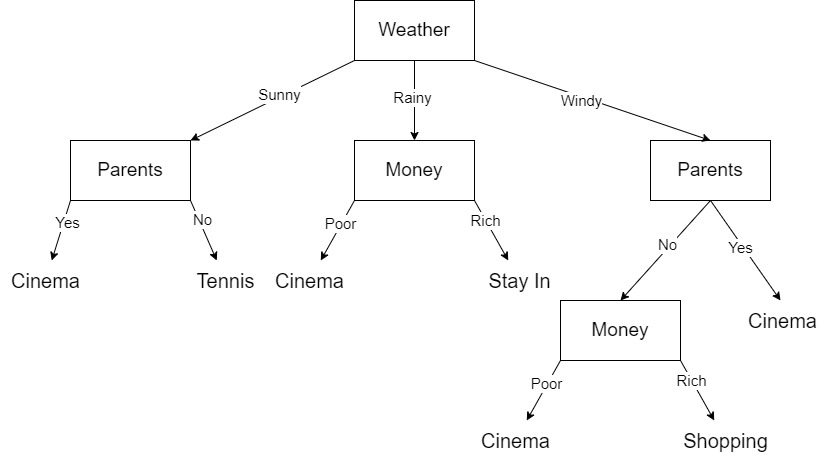
\includegraphics[scale=0.5]{figs/ID3_Q2_a}
		\end{figure}
	\textbf{\lr{Accuracy: 100\%}}
	\newpage
	\begin{latin}
		\subsection{Construct a decision tree model using only the first 6 samples from the
			dataset(W1 - W6). Evaluate the model's classification performance on
			these initial 6 samples as the training set. Then, use the model to classify
			the remaining samples in the dataset. What is the classification accuracy
			for both the training and test datasets? Discuss your findings and explain			the reasons behind the observed results.}
	\end{latin}
	\noindent
	\textbf{یادگیری با داده های آموزشی:}\\
	1 - \lr{Root Node}
	\begin{latin}
		\textbf{Decision}
		\begin{center}
			\begin{tabular}{|c|c|c|c|c|}
				\hline
				Cinema & Tennis & Stay in & Shopping\\
				\hline
				\hline
				4 & 1 & 1 & 0\\
				\hline
			\end{tabular}
		\end{center}
	\end{latin}
	\vspace{5pt}
	\[
	Entropy(S) = -\sum_{v \in S} p_v\log (p_v)
	\]
	\[
	Entropy(S) = -( \frac{4}{6} \times -0.59 + \frac{1}{6} \times -2.64 + \frac{1}{6} \times -2.64) = 1.23
	\]
	\begin{latin}
		\textbf{Money}
		\begin{center}
			\begin{tabular}{|c|c|c|c|c|c|}
				\hline
				Value & Cinema & Tennis & Stay in & Shopping\\
				\hline
				\hline
				Rich & 2 & 1 & 1 & 0\\
				\hline
				Poor & 2 & 0 & 0 & 0\\
				\hline
			\end{tabular}
		\end{center}
	\end{latin}
	\vspace{5pt}
	\[
	Entropy(S_{\text{\lr{v}}}) = -\sum_{v \in S} p_v\log (p_v)
	\]
	\[
	Entropy(S_{\tf{Rich}}) = -(\frac{2}{4} \times -1 + \frac{1}{4} \times -2 + \frac{1}{4} \times -2) = 1.5
	\]
	\[
	Entropy(S_{\tf{Poor}}) = -(\frac{2}{2} \times 0) = 0
	\]
	\vspace{10pt}
	\[
	Gain(S, \tf{Money}) = Entropy(S) - \sum_{v \in \tf{Money}} \frac{| S_v |}{| S |}Entropy(S_v)
	\] 
	\[
	\sum_{v \in \tf{Money}} \frac{| S_v |}{| S |}Entropy(S_v) = \frac{4}{6} \times 1.5 + \frac{2}{6} \times 0 = 1
	\]
	\[
	Gain(S, \tf{Money}) = 1.23 - 1 = 0.23
	\]
	\begin{latin}
		\textbf{Parents}
		\begin{center}
			\begin{tabular}{|c|c|c|c|c|c|}
				\hline
				Value & Cinema & Tennis & Stay in & Shopping\\
				\hline
				\hline
				Yes & 4 & 0 & 0 & 0\\
				\hline
				No &0& 1 & 1 & 0\\
				\hline
			\end{tabular}
		\end{center}
	\end{latin}
	\vspace{5pt}
	\[
	Entropy(S_{\tf{v}}) = -\sum_{v \in S} p_v\log (p_v)
	\]
	\[
	Entropy(S_{\tf{Yes}}) = -(\frac{4}{4} \times 0) = 0
	\]
	\[
	Entropy(S_{\tf{No}}) = -(\frac{1}{2} \times -1 + \frac{1}{2} \times -1) = 1
	\]
	\vspace{10pt}
	\[
	Gain(S, \tf{Parents}) = Entropy(S) - \sum_{v \in \tf{Parents}} \frac{| S_v |}{| S |}Entropy(S_v)
	\] 
	\[
	\sum_{v \in \tf{Parents}} \frac{| S_v |}{| S |}Entropy(S_v) = \frac{4}{6} \times 0 + \frac{2}{6} \times 1 = 0.33
	\]
	\[
	Gain(S, \tf{Parents}) = 1.23 - 0.33 = 0.9
	\]
	\begin{latin}
		\textbf{Weather}
		\begin{center}
			\begin{tabular}{|c|c|c|c|c|c|}
				\hline
				Value & Cinema & Tennis & Stay in & Shopping\\
				\hline
				\hline
				Sunny & ‌1& 1 & 0 & 0\\
				\hline
				Windy & 1 & 0 & 0 & 0\\
				\hline
				Rainy & 2 & 0 & 1 & 0\\
				\hline
			\end{tabular}
		\end{center}
	\end{latin}
	\vspace{5pt}
	\[
	Entropy(S_{\tf{v}}) = -\sum_{v \in S} p_v\log (p_v)
	\]
	\[
	Entropy(S_{\tf{Sunny}}) = -(\frac{1}{2} \times -1 + \frac{1}{2} \times -1) = 1
	\]
	\[
	Entropy(S_{\tf{Windy}}) = -(\frac{1}{1} \times 0) = 0
	\]
	\[
	Entropy(S_{\tf{Rainy}}) = -(\frac{2}{3} \times -0.59 + \frac{1}{3} \times -1.59) = 0.92
	\]
	\vspace{10pt}
	\[
	Gain(S, \tf{Weather}) = Entropy(S) - \sum_{v \in \tf{Weather}} \frac{| S_v |}{| S |}Entropy(S_v)
	\] 
	\[
	\sum_{v \in \tf{Weather}} \frac{| S_v |}{| S |}Entropy(S_v) = \frac{2}{6} \times 1 + \frac{1}{6} \times 0 + \frac{3}{6} \times 0.92 = 0.79
	\]
	\[
	Gain(S, \tf{Weather}) = 1.23 - 0.79 = 0.44
	\]
	\begin{latin}
		\textbf{Picking The Best Attribute}
		\begin{center}
			\begin{tabular}{|c|c|}
				\hline
				Attribute & Information Gain\\
				\hline
				\hline
				Money & 0.23\\
				Parents & 0.9\\
				Weather & 0.44\\
				\hline
			\end{tabular}
		\end{center}
	\end{latin}
	ویژگی انتخابی،
	\lr{Parents}
	می‌باشد.\\
	2 - \lr{(Parents - No) Node}
	\begin{latin}
		\textbf{Decision}
		\begin{center}
			\begin{tabular}{|c|c|c|c|c|}
				\hline
				Cinema & Tennis & Stay in & Shopping\\
				\hline
				\hline
				0 & 1 & 1 & 0\\
				\hline
			\end{tabular}
		\end{center}
		For $W_2, W_5$
	\end{latin}
	\vspace{5pt}
	\[
	Entropy(S) = -\sum_{v \in S} p_v\log (p_v)
	\]
	\[
	Entropy(S) = -( \frac{1}{2} \times -1 + \frac{1}{2} \times -1) = 1
	\]
	\begin{latin}
		\textbf{Money}
		\begin{center}
			\begin{tabular}{|c|c|c|c|c|c|}
				\hline
				Value & Cinema & Tennis & Stay in & Shopping\\
				\hline
				\hline
				Rich & 0 & 1 & 1 & 0\\
				\hline
				Poor & 0 & 0 & 0 & 0\\
				\hline
			\end{tabular}
		\end{center}
	\end{latin}
	\vspace{5pt}
	\[
	Entropy(S_{\text{\lr{v}}}) = -\sum_{v \in S} p_v\log (p_v)
	\]
	\[
	Entropy(S_{\tf{Rich}}) = -(\frac{1}{2} \times -1 + \frac{1}{2} \times -1) = 1
	\]
	\[
	Entropy(S_{\tf{Poor}}) = -(0 \times 0) = 0
	\]
	\vspace{10pt}
	\[
	Gain(S, \tf{Money}) = Entropy(S) - \sum_{v \in \tf{Money}} \frac{| S_v |}{| S |}Entropy(S_v)
	\] 
	\[
	\sum_{v \in \tf{Money}} \frac{| S_v |}{| S |}Entropy(S_v) = \frac{2}{2} \times 1= 1
	\]
	\[
	Gain(S, \tf{Money}) = 1 - 1 = 0
	\]
	\begin{latin}
		\textbf{Weather}
		\begin{center}
			\begin{tabular}{|c|c|c|c|c|c|}
				\hline
				Value & Cinema & Tennis & Stay in & Shopping\\
				\hline
				\hline
				Sunny & ‌0& 1 & 0 & 0\\
				\hline
				Windy & 0 & 0 & 0 & 0\\
				\hline
				Rainy & 0 & 0 & 1 & 0\\
				\hline
			\end{tabular}
		\end{center}
	\end{latin}
	\vspace{5pt}
	\[
	Entropy(S_{\tf{v}}) = -\sum_{v \in S} p_v\log (p_v)
	\]
	\[
	Entropy(S_{\tf{Sunny}}) = -(\frac{1}{1} \times 0) = 0
	\]
	\[
	Entropy(S_{\tf{Windy}}) = 0
	\]
	\[
	Entropy(S_{\tf{Rainy}}) = -(\frac{1}{1} \times 0) = 0
	\]
	\vspace{10pt}
	\[
	Gain(S, \tf{Weather}) = Entropy(S) - \sum_{v \in \tf{Weather}} \frac{| S_v |}{| S |}Entropy(S_v)
	\] 
	\[
	\sum_{v \in \tf{Weather}} \frac{| S_v |}{| S |}Entropy(S_v) = \frac{1}{2} \times 0 + \frac{1}{2} \times 0 = 0
	\]
	\[
	Gain(S, \tf{Weather}) = 1 - 0 = 1
	\]
	\begin{latin}
		\textbf{Picking The Best Attribute}
		\begin{center}
			\begin{tabular}{|c|c|}
				\hline
				Attribute & Information Gain\\
				\hline
				\hline
				Money & 0\\
				Weather & 1\\
				\hline
			\end{tabular}
		\end{center}
	\end{latin}
	ویژگی انتخابی،
	\lr{Weather}
	می‌باشد.
	
	\vspace{10pt}
	\textbf{دقت مدل روی داده‌های آموزشی}
	\[
	Accuracy_{\tf{Train}} = \frac{\tf{Correctly Labeled}}{\tf{All train samples}} = \frac{6}{6} = 100\%
	\]
	\vspace{10pt}
	\textbf{دقت مدل روی داده‌های تست}
	\[
	Accuracy_{\tf{Test}} = \frac{\tf{Correctly Labeled}}{\tf{All test samples}} = \frac{2}{4} = 50\%
	\]
	\textbf{شکل درخت تصمیم:}
	
	\begin{figure}[h!]
		\centering
		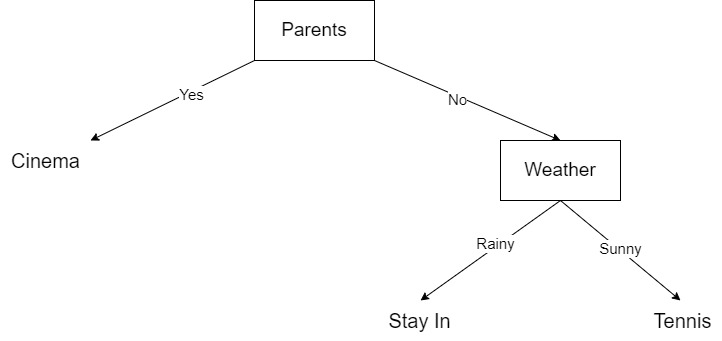
\includegraphics[scale=0.5]{figs/ID3_Q2_c}
	\end{figure}
	به نظر می‌رسد یکی از دلایل اصلی افت مقدار دقت در داده های تست، نبود نمونه‌هایی با مقادیر مختلف برای ویژگی‌ها در داده‌های آموزش بوده است، برای مثال برای مقدار 
	\lr{Windy}
	هیچ پیشبینی را نمی‌توان انجام داد زیرا مدل آن را تا الان بیرون از تسلط ویژگی 
	\lr{Parents}
	ندیده است.
	\begin{latin}
		\subsection{In scenarios where only a limited number of labeled examples are
			available for training (and no extra data is available for testing or
			validation), propose a specific pruning technique that could be integrated
			into the decision tree algorithm to prevent overfitting. Justify why you
			believe this technique would be effective.}
	\end{latin}
	با توجه به اینکه داده تستی نداریم، از این روش که بگذاریم درخت 
	\lr{overfit}
	کند و سپس 
	\lr{Post Pruning}
	به طریقی دیگر استفاده می‌کنیم.\\
	می‌توان در الگوریتم اضافه کرد، پس از اتمام کار، از هر برگ شروع میکنیم و درصورتی که مقدار آنتروپی آن از آستانه ای کمتر بود، به راس والد رفته و اینکار را انجام می‌دهیم تا جایی که این اتفاق نیفتد، سپس از آن راس که آنتروپی آن  دیگر کمتر از مقدار آستانه نیست، زیر درخت آن راس را حذف می‌کنیم تا از بیش برازش جلوگیری به عمل آمده و قابلیت تعمیم پذیری مدل بالاتر رود.
\end{document}